\section{Systemarchitektur und Rahmenbedingungen}

Die Konzeption eines Empfehlungssystems für den produktiven Einsatz bei der SV-Gruppe erfordert eine Architektur, die klar definierten Rahmenbedingungen gerecht wird. 
Aus dem Anwendungsfall ergeben sich eine Reihe von \ac{NFR}s, die die technische Ausgestaltung maßgeblich beeinflussen.

\label{sec:nfr}
Für den initialen Proof-of-Concept wurden drei zentrale NFRs als erfolgskritisch identifiziert. 
Erstens muss das System eine hohe Performanz aufweisen und in der Lage sein, eine große Anzahl paralleler Anfragen effizient zu verarbeiten. 
Als konkretes \ac{SLO} wird eine Latenz im 95. Perzentil von unter 500 Millisekunden angestrebt. 
Zweitens ist die Skalierbarkeit der Architektur essenziell, um flexibel auf wachsende Nutzerzahlen und Datenmengen reagieren zu können, 
wie sie im dynamischen Umfeld eines Nachrichtenportals zu erwarten sind. Drittens muss eine einfache Integrierbarkeit gewährleistet sein, 
weshalb das System über eine standardisierte REST-API angebunden wird, um die Integration in bestehende Redaktions- und IT-Workflows zu erleichtern.

% \subsection{Sekundäre und zukünftige Anforderungen}
Obwohl es sich zunächst um einen Prototypen handelt, wurden weitere Anforderungen identifiziert, die für einen späteren, 
vollumfänglichen Produktivbetrieb relevant sind. Dazu gehören die Gewährleistung von Datenschutz und Sicherheit gemäß der \ac{DSGVO}, 
eine hohe Verfügbarkeit und Ausfallsicherheit zur Sicherstellung eines unterbrechungsfreien Betriebs sowie die Transparenz der Empfehlungslogik, 
um das Vertrauen der Nutzer zu fördern. Diese Aspekte wurden im aktuellen Entwurf bereits konzeptionell berücksichtigt.

\subsection{Rahmenbedingungen}

Die bestehende IT-Infrastruktur der SV-Gruppe, die auf der \ac{GCP} basiert, definiert die zentralen Rahmenbedingungen für dieses Projekt. 
Der gesamte Artikelkorpus sowie die aus \ac{GA4} stammenden Nutzerinteraktionsdaten liegen zentral in BigQuery-Tabellen vor. 
Eine entscheidende Ressource stellen hochdimensionale (3072D) Artikel-Embeddings dar, 
welche aus den Titeln und Texten der Artikel generiert wurden. Aufgrund ihrer bewährten Effektivität in verwandten Anwendungsfällen, 
wie der semantischen Anzeigenausspielung, werden diese Embeddings auch im Rahmen dieser Arbeit genutzt.

% \subsection{Technologische Architektur}
\begin{figure}[htbp]
    \centering
    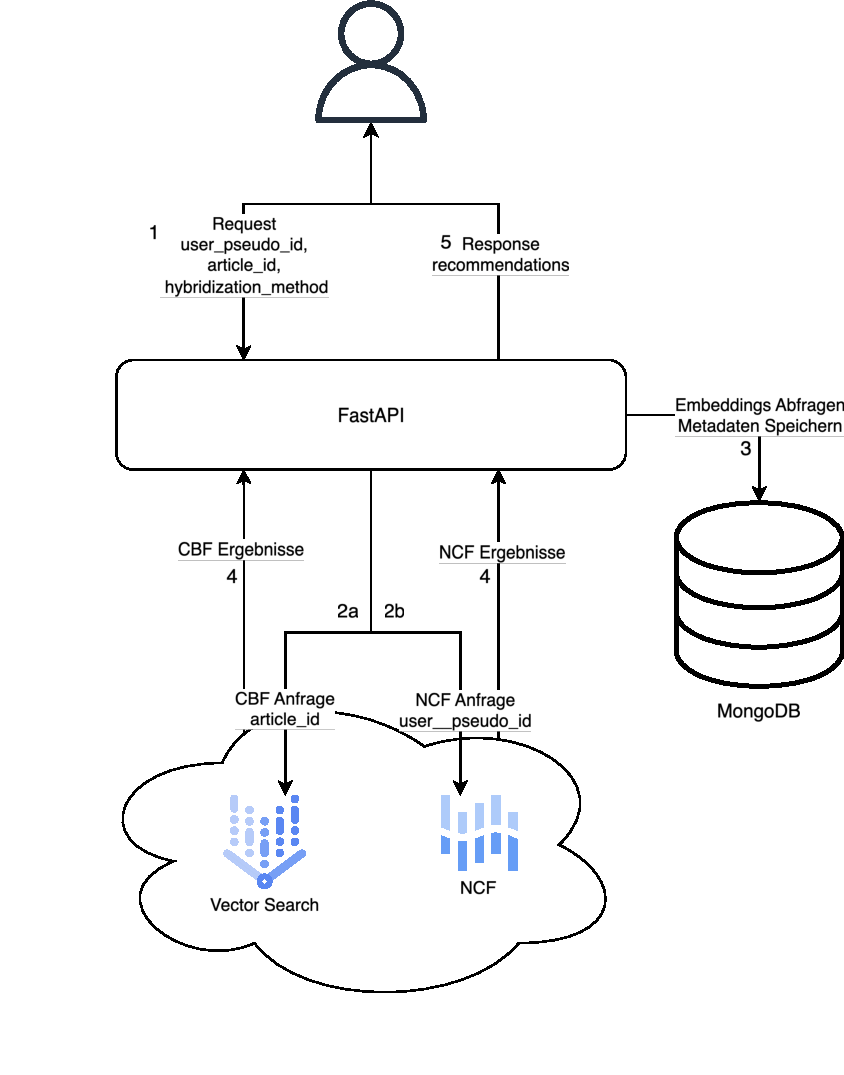
\includegraphics[width=0.6\textwidth]{content/figures/svg/architektur.pdf}
    \caption{Die technologische Architektur des hybriden Empfehlungssystems. Der nummerierte Datenfluss zeigt den Weg einer Anfrage vom Nutzer (1), 
    über die parallelen Abfragen an die ML-Dienste (2a, 2b) und die Datenbank (3), die eintreffenden Ergebnisse (4) bis zur finalen Empfehlung (5).}
    \label{fig:architektur}
\end{figure}
Die technologische Architektur ist als cloud-nativer Microservice-Ansatz auf der \ac{GCP} konzipiert,
um die in Abschnitt \ref{sec:nfr} definierten Anforderungen an Skalierbarkeit und Performanz zu erfüllen. 
Als zentraler Orchestrator dient ein in Python implementierter Service, der auf dem performanten FastAPI-Framework basiert. 
Dieser Service ist nicht nur für die Entgegennahme von Anfragen und die Steuerung der Modell-Endpunkte verantwortlich, 
sondern auch für die Hybridisierung der Empfehlungsergebnisse. Das Design wurde modular gestaltet, 
um zukünftig auch fortgeschrittenere Hybridisierungsstrategien integrieren zu können.

% \subsubsection{API-Design und Orchestrierung}
\label{sec:api_design}

Das Herzstück des Systems bildet der API-Service, welcher die Schnittstelle nach außen darstellt und die interne Logik steuert. 
Die API wird über einen REST-Endpunkt unter der Adresse \texttt{/v1/recommendations} bereitgestellt und kommuniziert über einen 
JSON-basierten Datenvertrag. Eine Anfrage an den Dienst enthält die \texttt{user\_pseudo\_id}, die \texttt{article\_id} 
als Kontext sowie die gewünschte Hybridisierungsstrategie. 

Die Implementierung basiert auf dem Python-Framework FastAPI, das aufgrund seiner hohen asynchronen Leistungsfähigkeit durch das \ac{ASGI} und 
der automatischen Generierung interaktiver Dokumentation ausgewählt wurde. Der Service orchestriert bei 
jeder Anfrage die parallelen Abfragen an die untergeordneten ML-Dienste und die Datenbank, führt die Ergebnisse zusammen 
und wendet die Logik zur Hybridisierung an, bevor die finale Empfehlungsliste an den Client zurückgesendet wird.

% \subsubsection{Content-Based Filtering mittels Vektorsuche}
\label{sec:cbf_service}

Die technische Umsetzung des \ac{CBF}-Ansatzes erfolgt mittels der Vertex AI Vektorsuche. 
Das Finden der thematisch ähnlichsten Artikel zu einem gegebenen Beitrag ist ein Nearest-Neighbor-Problem
im hochdimensionalen Vektorraum. 
Eine exakte Brute-Force-Suche über den gesamten Datenbestand ist für Echtzeitanwendungen mit geringer Latenz rechentechnisch nicht durchführbar.

Daher setzt Vertex AI Vektorsuche auf einen \ac{ANN}-Algorithmus. 
Dieser Ansatz tauscht eine geringfügige Einbuße an Genauigkeit gegen einen massiven Gewinn an Abfragegeschwindigkeit. 
Die zugrundeliegende Technologie ist Googles \ac{ScaNN}-Algorithmus, der im Kern auf zwei Prinzipien basiert:

\begin{itemize}
    \item \textbf{Partitionierung des Vektorraums:} Der Index unterteilt den hochdimensionalen Raum in eine Vielzahl von Clustern oder Zellen. 
    Bei einer Suchanfrage müssen dann nicht mehr alle Vektoren durchsucht werden, sondern nur noch die Vektoren in den wahrscheinlichsten Partitionen.
    \item \textbf{Vektorquantisierung:} Innerhalb dieser Partitionen werden die Vektoren durch eine Form der intelligenten Komprimierung repräsentiert, 
    um den Speicherbedarf zu reduzieren und Distanzberechnungen zu beschleunigen. Google setzt hierbei auf fortgeschrittene Methoden wie die anisotrope 
    Vektorquantisierung, um den Informationsverlust bei der Komprimierung zu minimieren \cite{avq_2020}.
\end{itemize}

Der ScaNN-Algorithmus lernt, die vielversprechendsten Partitionen für eine gegebene Anfrage effizient zu identifizieren und führt dann innerhalb 
dieser Partitionen eine schnelle Distanzberechnung auf den quantisierten Vektoren durch. 
Die Forschung zur Optimierung dieser Indexierungsstrategien entwickelt sich stetig weiter, wie das Paper zu SOAR zeigt, 
einem Nachfolger-Ansatz zur Verbesserung der Indexeffizienz \cite{soar_2023}.

% \subsubsection{Neural Collaborative Filtering}
\label{sec:ncf_service}

Als kollaborativer Filteransatz wird in dieser Arbeit das \ac{NCF}-Modell eingesetzt. 
Traditionelle Ansätze wie die \ac{MF} modellieren die Interaktion zwischen Nutzern und Artikeln durch ein einfaches Skalarprodukt ihrer latenten Vektoren,
was die Ausdrucksstärke des Modells auf lineare Zusammenhänge limitiert.

Das NCF-Framework generalisiert diesen Ansatz, indem es das Skalarprodukt durch eine neuronale Architektur ersetzt. 
Konkret wird ein \ac{MLP} genutzt, um eine beliebige, auch nicht-lineare Interaktionsfunktion direkt aus den Daten zu erlernen \cite{he_neural_2017}. 
Diese Fähigkeit, komplexe Muster im Nutzer-Item-Interaktionsverhalten zu erfassen, macht das NCF-Modell zu einer 
leistungsfähigen Wahl für die Generierung personalisierter Empfehlungen.
Für den produktiven Einsatz wird das trainierte Modell auf einem dedizierten Vertex AI Endpoint bereitgestellt, 
um skalierbare Echtzeit-Inferenzen für gegebene Nutzer-IDs zu ermöglichen.

\subsection{Datenbasis und Einschränkungen}
\label{sec:data}
Der für das \ac{NCF}-Modell zugrundeliegende Datensatz SM-News-Jan25 bezieht sich ausschließlich auf \ac{GA4}-Daten vom Januar 2025.
Der Grund für diese Einschränkung liegt in den Kosten des Modelltrainings für große Datensätze. Für das Training werden die ersten drei Wochen 
und für den Test die letzte Woche des SM-News-Jan25 genutzt. 

Eine zentrale Eigenschaft des Datensatzes ist seine stark rechtsverschobene Verteilung, 
sowohl bei der Artikelpopularität als auch bei der Nutzeraktivität. Dieses als Long-Tail-Verteilung 
bekannte Phänomen ist typisch für Mediendaten und stellt eine Kernherausforderung für Empfehlungssysteme dar \cite{wu_personalized_2022, raza_news_2020}.

% content/figures/plot_artikelverteilung_train.tex

\begin{figure}[H]
    \centering
    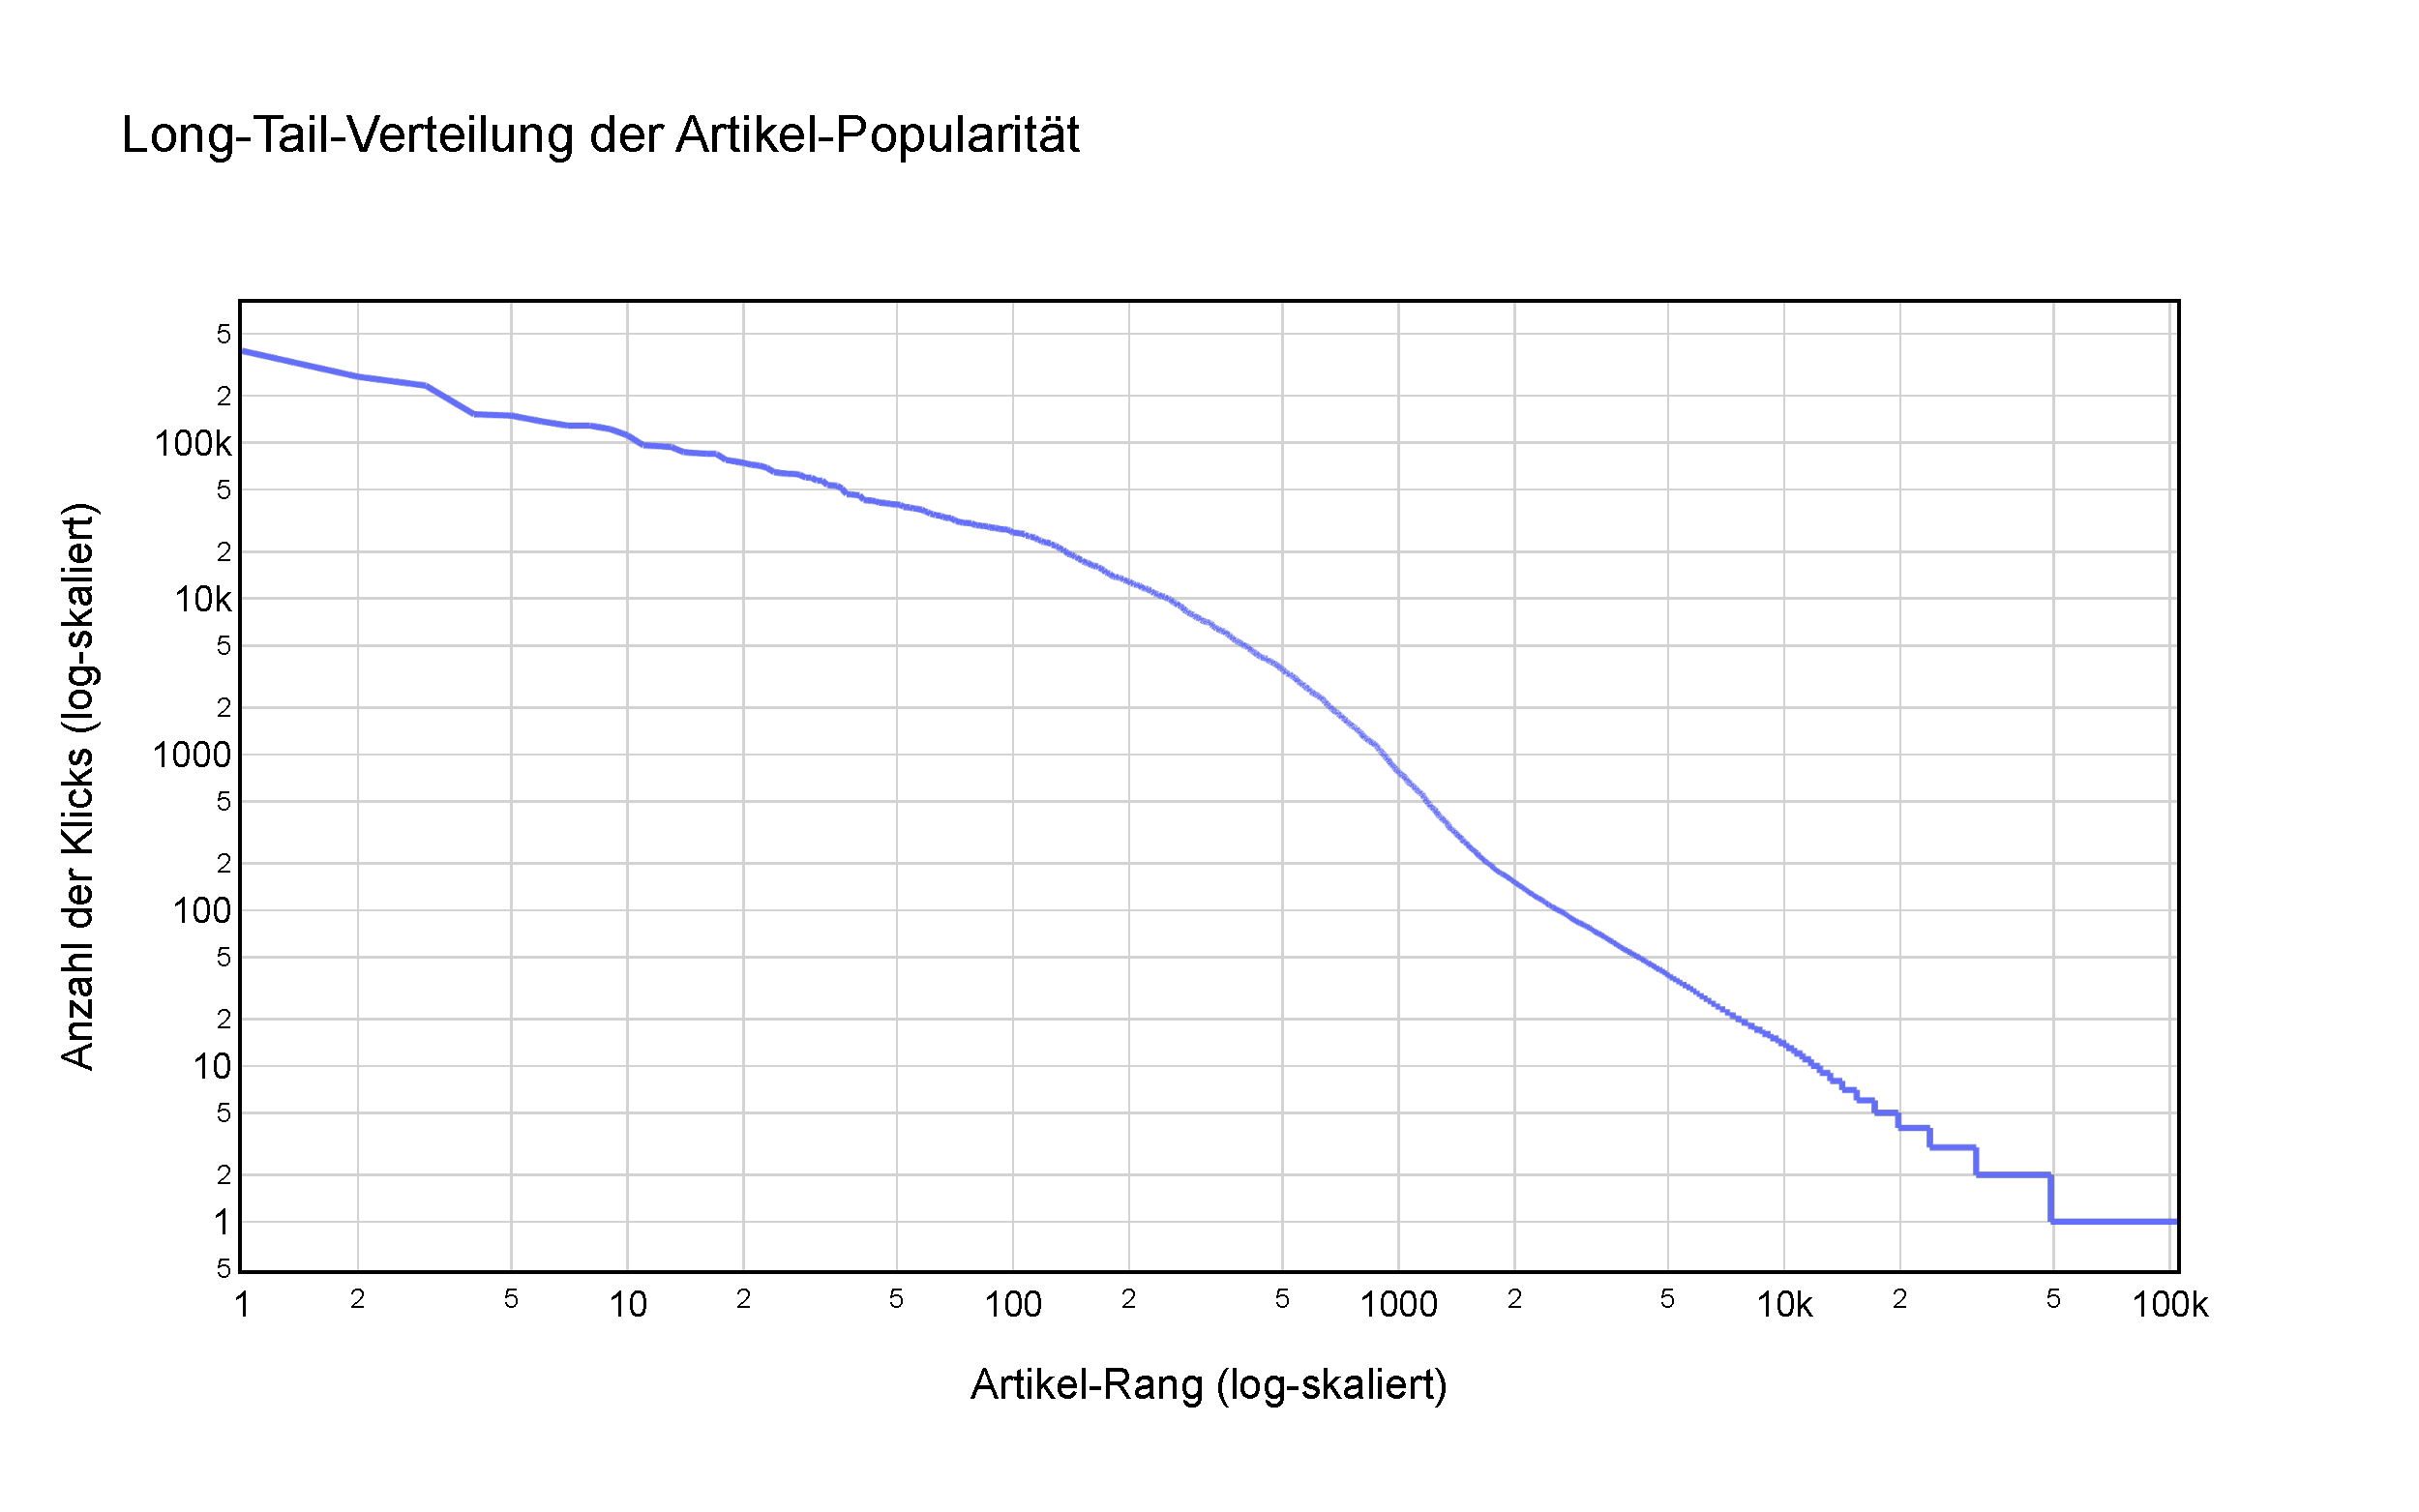
\includegraphics[width=0.9\textwidth]{content/figures/svg/artikel_verteilung_train.pdf}
    \caption{Popularitätsverteilung der Artikel im Trainingsdatensatz. Die Grafik zeigt, dass eine geringe Anzahl von Artikeln einen Großteil der Klicks auf sich vereint, während die Mehrheit der Artikel nur wenige Interaktionen erhält (Long-Tail).}
    \label{fig:artikelverteilung_train}
\end{figure}

\newpage
Die Verteilung manifestiert sich in zwei Dimensionen:

\begin{itemize}
    \item 
    \textbf{Artikelpopularität:} Wie in Abbildung~\ref{fig:artikelverteilung_train} dargestellt,\newline 
    konzentriert sich ein 
    überproportional großer Anteil der Seitenaufrufe auf eine sehr kleine Gruppe von viralen "Hit"-Artikeln, die den "Kopf" der Verteilung bilden. 
    Dies wird durch die kurze Lebensdauer von Nachrichtenartikeln zusätzlich verstärkt.
    \item \textbf{Nutzeraktivität:} Ein analoges Muster zeigt sich beim Nutzerverhalten. 
    Eine kleine Kohorte von hochaktiven "Power-Nutzern" ist für einen Großteil der Klick-Events verantwortlich, während die Mehrheit der Nutzer nur 
    sporadisch mit wenigen Klicks interagiert.
\end{itemize}

Diese ungleiche Verteilung führt zu einem inhärenten Popularity Bias in den Daten. 
Naive Modelle neigen dazu, allen Nutzern wiederholt dieselben populären Bestseller-Artikel zu empfehlen, 
was das Ziel der Personalisierung untergräbt und die Gefahr birgt, Nutzer in einer Filterblase zu isolieren. 
Gleichzeitig entsteht ein Kaltstart-Problem für Nischen-Artikel im Long Tail, die kaum eine Chance haben, empfohlen zu werden. 
Eine zentrale Herausforderung dieser Arbeit ist daher die Konzeption eines Systems, 
das diesen Popularity Bias aktiv ausbalanciert, um auch relevante Nischeninhalte an die passenden Nutzer auszuspielen.

% content/figures/plot_nutzerverteilung_train.tex

\begin{figure}[H]
    \centering
    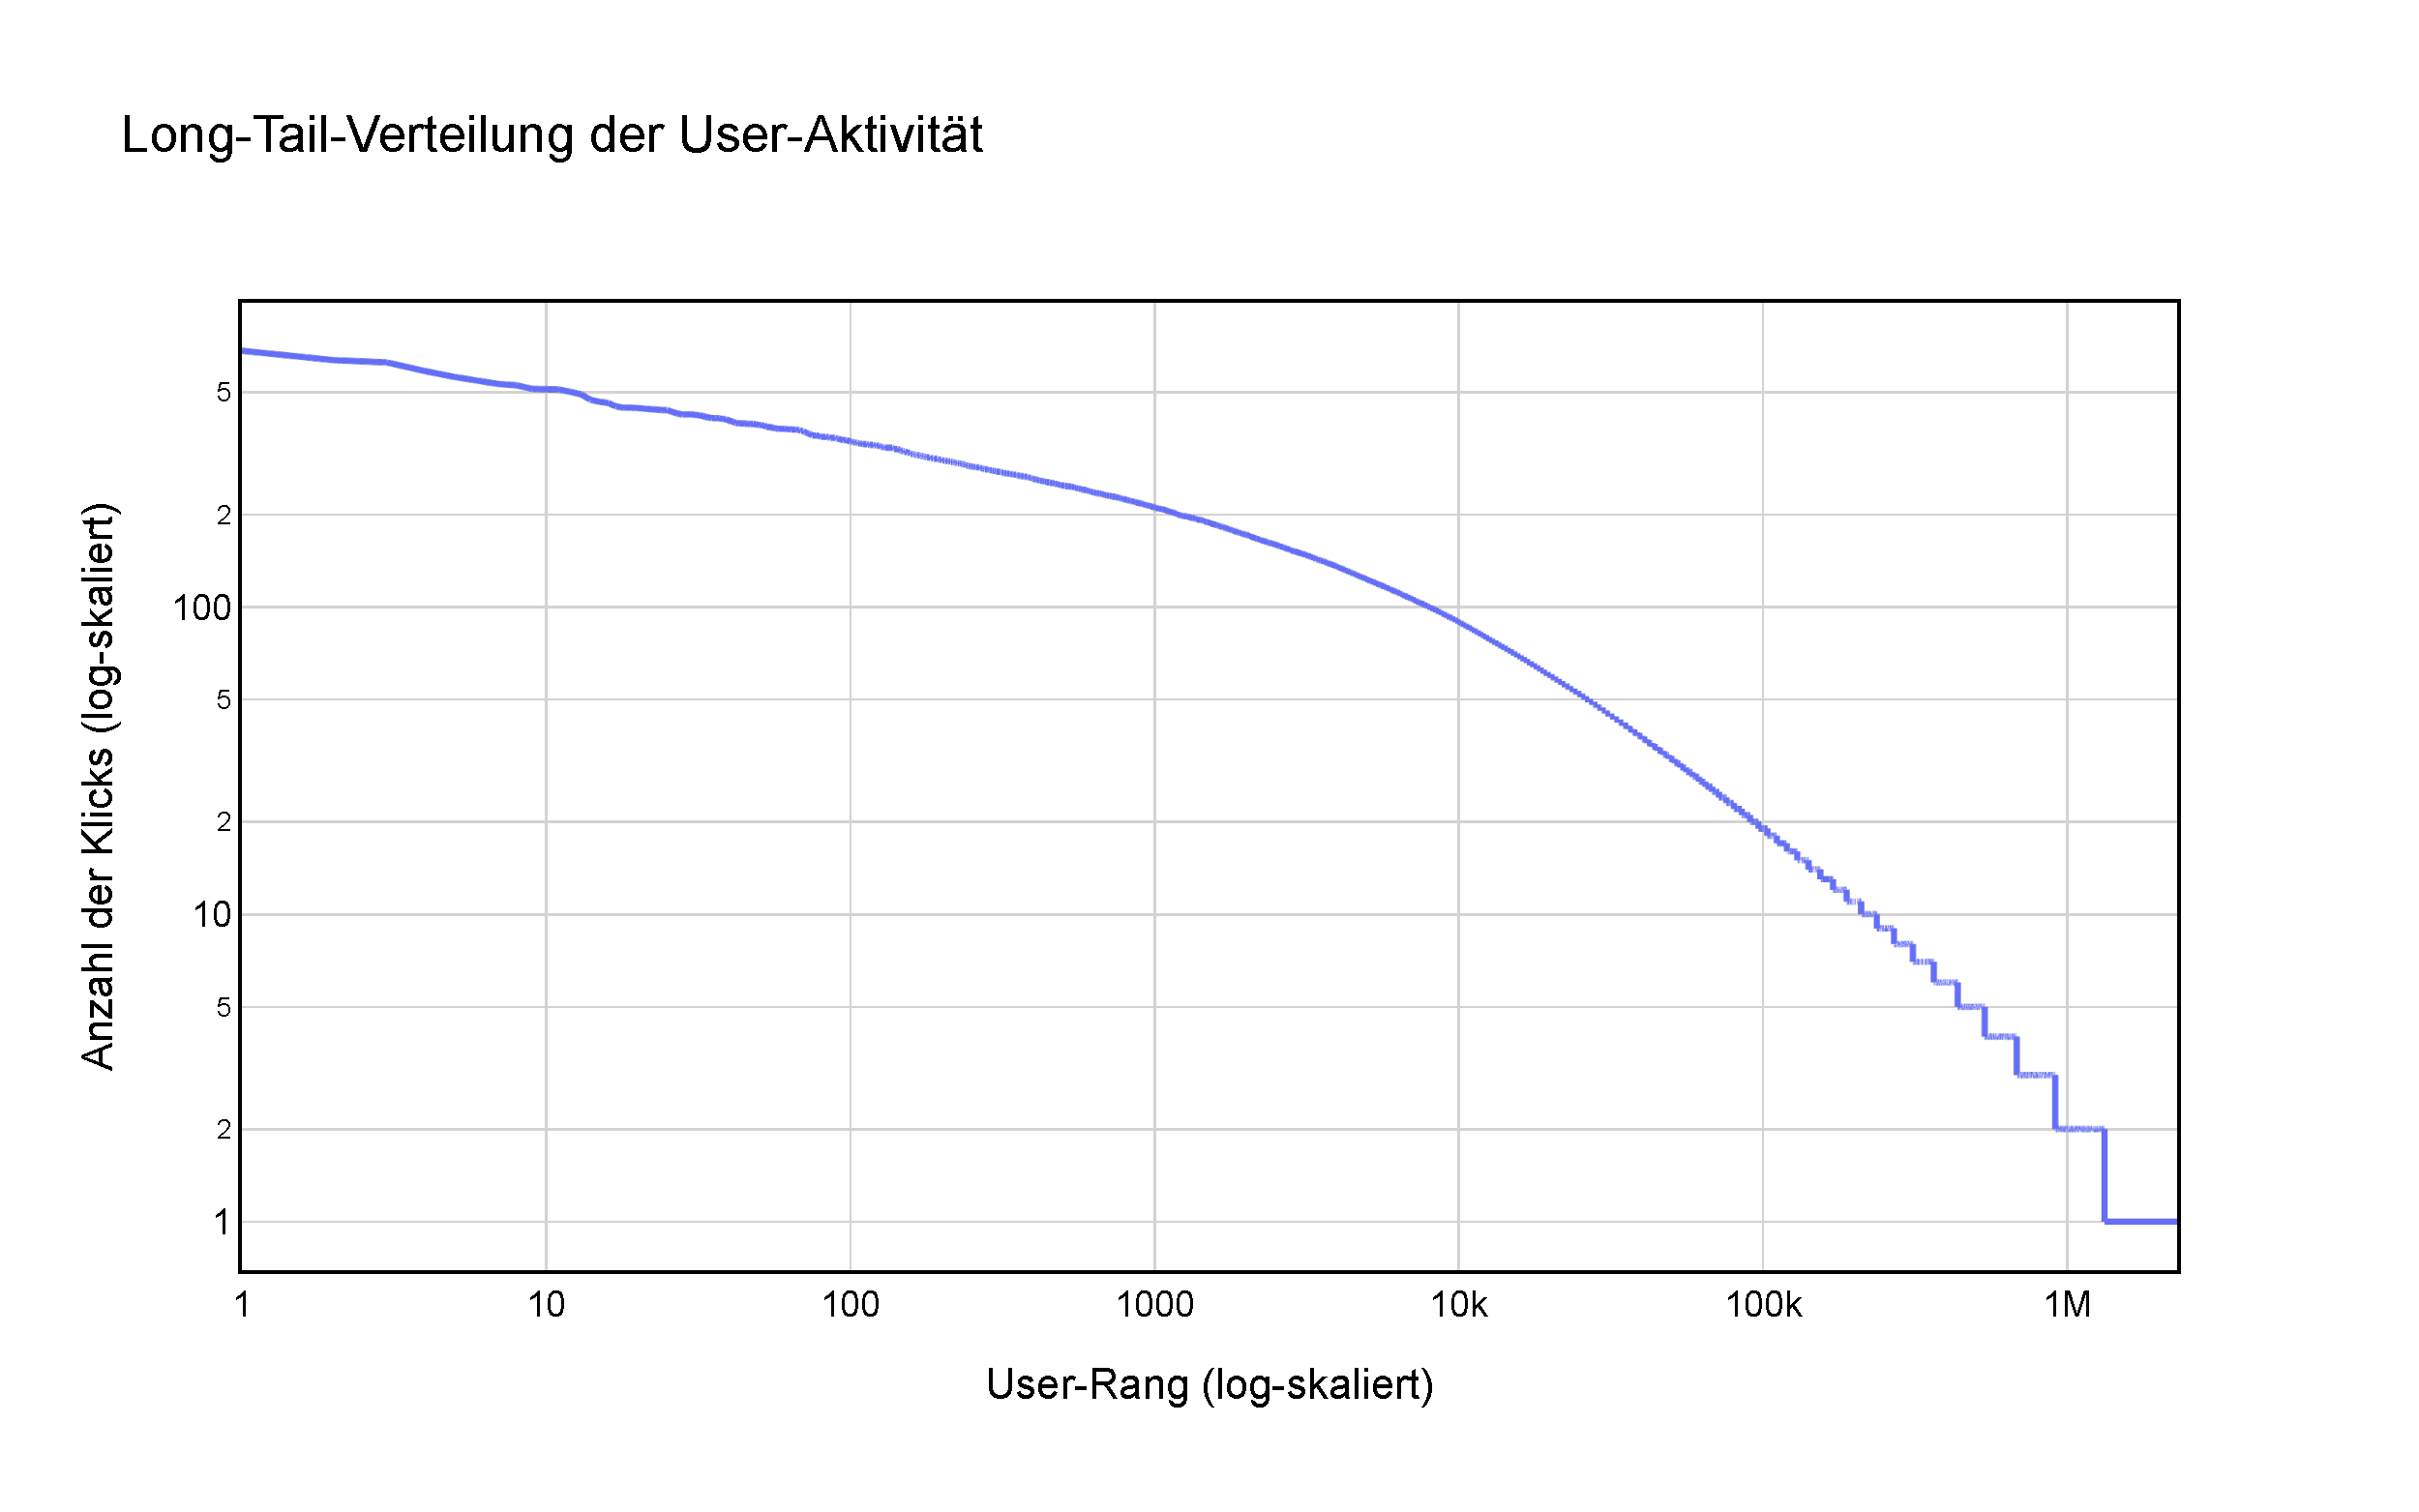
\includegraphics[width=0.9\textwidth]{content/figures/svg/nutzer_verteilung_train.pdf}
    \caption{Verteilung der Nutzeraktivität im Trainingsdatensatz. Die Darstellung verdeutlicht die typische Long-Tail-Verteilung: Eine große Anzahl von Nutzern interagiert nur selten mit Artikeln, während eine kleine Gruppe von "Power-Nutzern" für einen Großteil der Klicks verantwortlich ist.}
    \label{fig:nutzerverteilung_train}
\end{figure}

Die zugrundeliegenden statistischen Kennzahlen des Trainingsdatensatzes sind in Tabelle~\ref{tab:train_stats} zusammengefasst.

% content/tables/statistiken_trainingsdaten.tex

\begin{table}[H]
    \centering
    \caption{Statistische Kennzahlen des Trainingsdatensatzes, basierend auf den Klick-Logs der ersten drei Januarwochen.}
    \label{tab:statistiken_training}
    \begin{tabular}{lr}
        \toprule
        \textbf{Metrik} & \textbf{Wert} \\
        \midrule
        Gesamte Interaktionen (Klicks) & 11.412.116 \\
        Einzigartige user\_pseudo\_ids & 2.294.733 \\
        Einzigartige Artikel & 104.462 \\
        \bottomrule
    \end{tabular}
\end{table}
\label{tab:train_stats}

Um die Klick-Events für das \ac{NCF}-Modell nutzbar zu machen, wurden sie in eine User-Item-Interaktionsmatrix überführt. 
Dabei repräsentieren die Zeilen die einzigartigen Nutzer und die Spalten die einzigartigen Artikel des Trainingszeitraums. 
Eine Zelle $(i, j)$ in der Matrix erhält den Wert 1, wenn der Nutzer $i$ mit dem Artikel $j$ interagiert hat, andernfalls den Wert 0. 
Dieser Prozess resultiert in einer binären Matrix, die das implizite Feedback der Nutzer abbildet.

Die resultierende Matrix weist mit Dimensionen von circa 2,3 Millionen Nutzern und 104.000 Artikeln eine Dichte von unter 0,005\,\% auf. 
Ihre entscheidende Eigenschaft ist daher ihre extreme Dünnbesetzung. 
Diese Sparsity ist eine typische Herausforderung für \ac{CF}-Modelle, da für jeden Nutzer nur eine verschwindend geringe Anzahl an Interaktionen im Verhältnis zur Gesamtmenge der Artikel vorliegt. 
Dies erschwert es dem Modell, aussagekräftige Muster im Nutzerverhalten zu erlernen und auf neue User-Item-Paare zu generalisieren.

Bei der Interpretation der Ergebnisse müssen folgende Limitationen berücksichtigt werden:

\begin{itemize}
    \item \textbf{Zeitlicher Rahmen:} Der verwendete Datensatz deckt ausschließlich den Januar 2025 ab. 
    Dies stellt eine Momentaufnahme dar und verhindert, dass das Modell saisonale Effekte (z.B. Feiertage) oder langfristige Entwicklungen im Nutzerinteresse erfassen kann.

    \item \textbf{Implizites Feedback:} Als Interaktionssignal werden ausschließlich Klicks verwendet. 
    Diese Form des impliziten Feedbacks ist zwar reichlich vorhanden, aber mehrdeutig. 
    Ein Klick ist kein garantierter Indikator für Nutzerzufriedenheit; er kann auch zu einem sofortigen Verlassen der Seite (Bounce) führen. 
    Andere Signale wie die Verweildauer wurden in diesem Prototypen nicht berücksichtigt.

    \item \textbf{Offline-Evaluation:} Die Modellgüte wird offline anhand historischer Daten mit Metriken wie dem \ac{nDCG} evaluiert. 
    Diese Methodik kann die tatsächliche Auswirkung auf das Nutzerverhalten im Live-Betrieb nicht vollständig abbilden. 
    Um den realen Business Impact auf KPIs wie Sitzungsdauer oder Nutzerbindung zu messen, wäre ein abschließender Online-A/B-Test der nächste logische Schritt.
\end{itemize}
